\documentclass{standalone}

\usepackage{tikz}
\usepackage{circuitikz}

\tikzset{block/.style = {draw, fill=white, very thick, rectangle, minimum height=1cm, minimum width=2cm},
         lblock/.style={draw,fill=white,very thick, rectangle, minimum height=3cm, minimum width=1cm},
         sum/.style= {draw, fill=white, very thick, circle, node distance=0.5cm}}

         
\begin{document}
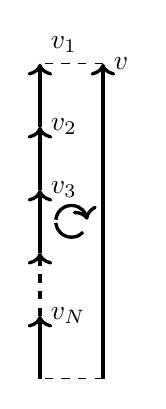
\begin{tikzpicture}[scale=4]
    \draw[->,very thick](0,0)--(0,0.2)node[right]{$v_N$};
    \draw[dashed, ->,very thick](0,0.2)--(0,0.4);
    \draw[->,very thick](0,0.4)--(0,0.6)node[right]{$v_3$};
    \draw[->,very thick](0,0.6)--(0,0.8)node[right]{$v_2$};
    \draw[->,very thick](0,0.8)--(0,1)node[above right]{$v_1$};
    \draw[->,very thick](0.2,0)--(0.2,1)node[right]{$v$};
    \draw[dashed](0.2,0)--(0,0);
    \draw[dashed](0.2,1)--(0,1);

    \draw[->,very thick]plot[smooth, domain=0.05:0.15](\x,{0.5+(0.0025-(\x-0.1)^2)^0.5});
    \draw[-,very thick]plot[smooth, domain=0.05:0.137](\x,{0.5-(0.0025-(\x-0.1)^2)^0.5});
\end{tikzpicture}
\end{document}